\Subsection{Билет 99: Алгебра и σ-алгебра множеств. Определе-
ние, свойства, примеры. Теорема о существовании
минимальной σ-алгебры содержащей данное семейство множеств. Борелевская оболочка и борелевские множества.}

Все рассматриваемые далее мн-ва - подмножества некоторого фиксированного мн-ва $X$.

\begin{definition}[Обозначение]\thmslashn
	
	$A \sqcup B$ -- дизъюнктное объединение.
	
	$A\cap B = \emptyset$ и $A\sqcup B := A\cup B$
\end{definition}

\begin{remark}[-- напоминание]\thmslashn
	
	$A\setminus \bigcup\limits_{\alpha \in I} B_{\alpha} = \bigcap\limits_{\alpha \in I} (A\setminus B_{\alpha})$
	
	$A\setminus \bigcap\limits_{\alpha \in I} B_{\alpha} = \bigcup\limits_{\alpha \in I} (A\setminus B_{\alpha})$

\end{remark}

\begin{definition}\thmslashn

	Будет рассматривать некие семейства множеств $\mathcal{A} \subset 2^X$

\end{definition}

\begin{properties}[семейства множеств $\mathcal{A}$]\thmslashn
	
	\begin{itemize}
		
		\item[($\sigma_0$)] $A,B \in \mathcal{A} \implies A\cup B \in \mathcal{A}$
		
		\item[($\delta_0$)] $A,B \in \mathcal{A} \implies A\cap B \in \mathcal{A}$
		
		\item[($\sigma$)] $A_n \in \mathcal{A} \implies \bigcup\limits_{n=1}^{\infty} A_n \in \mathcal{A}$
		
		\item[($\delta$)] $A_n \in \mathcal{A} \implies \bigcap\limits_{n=1}^{\infty} A_n \in \mathcal{A}$
	\end{itemize}
\end{properties}

\begin{definition}\thmslashn

	$\mathcal{A}$ -- симметричная, если $A \in \mathcal{A} \implies \overline{A} \in \mathcal{A}$

\end{definition}


\begin{statement}\thmslashn
	
	$\mathcal{A}$ -- симметрично, то
	
	$(\sigma_0) \iff (\delta_0)$ и $(\sigma) \iff (\delta)$
\end{statement}

\begin{proof}\thmslashn
	
	$X\setminus (A\cup B) = (X\setminus A) \cap (X\setminus B)$
	
	
	$X\setminus \bigcup\limits_{n=1}^{\infty}A_n = \bigcap\limits_{n = 1}^{\infty} (X\setminus A_n)$
\end{proof}

\begin{definition}\thmslashn
	
	$\mathcal{A}$ -- алгебра множеств, если  $\emptyset \in \mathcal{A}$, $\mathcal{A}$ -- симметрично и обладает свойствами $(\delta_0)$ и $(\sigma_0)$.
	
	$\mathcal{A}$ -- $\sigma$-алгебра множеств, если  $\emptyset \in \mathcal{A}$, $\mathcal{A}$ -- симметрично и обладает свойствами $(\delta)$ и $(\sigma)$.
	
\end{definition}


\begin{properties}[алгебры множеств]\thmslashn
	
	\begin{enumerate}
		
		\item $\emptyset,X \in \mathcal{A}$
		
		\item $A,B \in \mathcal{A} \implies A\setminus B \in \mathcal{A}$
		
		\item $A_1,...,A_n \in \mathcal{A} \implies \bigcap\limits_{k=1}^n A_k $ и $\bigcup\limits_{k=1}^n A_k \in \mathcal{A}$
		
		
	\end{enumerate}
\end{properties}


\begin{proof}\thmslashn
	
	2. $A\setminus B = A \cap \overline{B}$
	
	3. прошлое утверждение + индукция
\end{proof}

\begin{example}\thmslashn
	
	\begin{enumerate}
		
		\item $\mathcal{A} = \{\emptyset, X \}$ -- $\sigma$-алгебра
		
		\item $2^X$ -- $\sigma$-алгебра
		
		\item $X = \R^n \;\;\; \mathcal{A}$ -- все ограниченные подмножества и их дополнения.
		
		$\mathcal{A}$ -- алгебра, но не $\sigma$-алгебра, ведь если взять объединение единичных клеточек подряд в одну строчку, то получится неограниченное мн-во, и дополнение будет тоже неограниченным.
		
		\item $\mathcal{A}$ -- алгебра ($\sigma$-алгебра) подмножеств $X$.
		
		$Y\subset X \;\; \mathcal{A}_Y := \{Y\cap A \;:\;\;A\in \mathcal{A} \}$
		
		$\mathcal{A}_Y$ --  алгебра ($\sigma$-алгебра) подмножеств $Y$.
		
		Это индуцированная алгебра ($\sigma$-алгебра) - ограничили структуру на подмножество.

		\item Пусть есть $\mathcal{A}_\alpha$ -- алгебры ($\sigma$-алгебры).  Тогда их пересечение -- алгебра ($\sigma$-алгебра).

		Действительно, понятно, что пустое лежит. Если лежит какое-то $A$, то оно лежит и во всех алгебрах, поэтому во всех алгебрах есть и дополнение $A$, поэтому оно есть и в пересечении.

		\item 
		$X\supset A,B$
		
		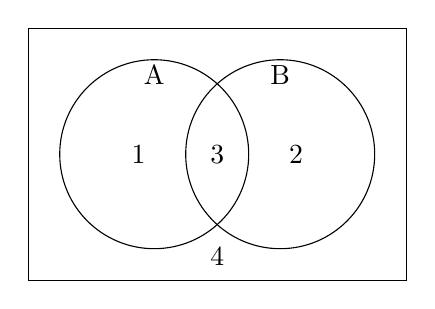
\begin{tikzpicture}[scale=0.4]
		\draw (0, 0) rectangle (12, 8);
		\draw (4, 4) circle (3);
		\draw (8, 4) circle (3);
		\node at (4, 6.5) {A};
		\node at (8, 6.5) {B};
		\node at (3.5, 4) {1};
		\node at (8.5, 4) {2};
		\node at (6, 4) {3};
		\node at (6, 0.75) {4};
		\end{tikzpicture}
		
		Все, что можем собрать из кусочков на картинке можно положить в семейство множеств.
		
		Кусочков $4$, итого $16$ множеств и это будет наименьшая $\sigma$-алгебра, содержащая множества $A$ и $B$. 

	\end{enumerate}
\end{example}

\begin{theorem}\thmslashn
	
	Для любой системы подмножеств $\mathcal{E}$ множества $X$ существует минимальная по включению алгебра ($\sigma$-алгебра), содержащая $\mathcal{E}$.
\end{theorem}


\begin{proof}\thmslashn
	
	Рассмотрим все $\sigma$-алгебры $\mathcal{A}_{\alpha}$, содержащие $\mathcal{E}$.
	
	Такие $\sigma$-алгебры точно существуют, т.к. например $2^X \supset \mathcal{E}$ и является $\sigma$-алгеброй.
	
	
	Рассмотрим $\mathcal{A} := \bigcap\limits_{\alpha\in I} \mathcal{A}_{\alpha} \supset \mathcal{E}$

	По пятому примеру, это $\sigma$-алгебра.
	
	Покажем, что это наименьшая по включению $\sigma$-алгебра, содержащая $\mathcal{E}$. Пусть $\mathcal{B}$ -- минимальная $\sigma$-алгебра, содержащая $\mathcal{E}$.
	
	Тогда $\exists \beta \in I  \;\;\; \mathcal{A}_{\beta} = \mathcal{B}$, но
	
	$\mathcal{A} = \bigcap\limits_{\alpha \in I} \mathcal{A}_{\alpha} \subset \mathcal{A}_{\beta} = \mathcal{B} \implies \mathcal{A} \subset \mathcal{B}$
\end{proof}

\begin{definition}\thmslashn
	
	$\mathcal{E}$ -- семейство подмножеств $X$.
	
	Борелевская оболочка $\mathcal{E} \;\;\;\; \mathcal{B}(\mathcal{E})$
	
	-- наименьшая $\sigma$-алгебра, содержащая $\mathcal{E}$
	
	
\end{definition}

\begin{definition}\thmslashn
	
	Борелевская $\sigma$-алгебра $\mathcal{B}^n$ -- минимальная $\sigma$-алгебра, содержащая все открытые множества в $\R^n$.
\end{definition}


\begin{remark}\thmslashn
	
	$\mathcal{B}^n \ne 2^{\R^n}$
	
	Более того, у них разные мощности. Первое -- континуально, второе еще больше. Но поймём мы это позже.
\end{remark}
